\subsection{Image\-Subtraction  Class Reference}
\label{class_imagesubtraction}\index{ImageSubtraction@{Image\-Subtraction}}
For subtracting images using the Alard kernel fit technique. A basic assumption: Ref and New are already geometrically aligned. 


{\tt \#include $<$imagesubtraction.h$>$}

Inheritance diagram for Image\-Subtraction::\begin{figure}[H]
\begin{center}
\leavevmode
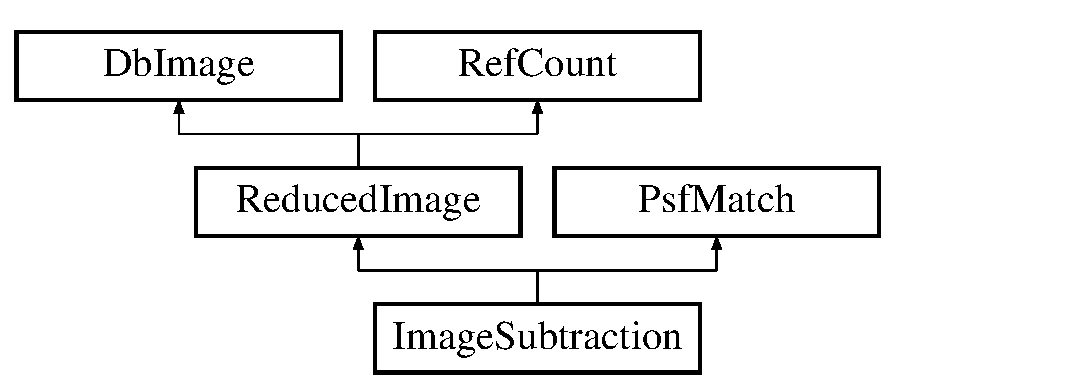
\includegraphics[height=3cm]{class_imagesubtraction}
\end{center}
\end{figure}
\subsubsection*{Public Methods}
\begin{CompactItemize}
\item 
\index{ImageSubtraction@{ImageSubtraction}!ImageSubtraction@{Image\-Subtraction}}\index{ImageSubtraction@{ImageSubtraction}!ImageSubtraction@{Image\-Subtraction}}
{\bf Image\-Subtraction} (const string \&Name, const {\bf Reduced\-Image} \&Ref\-Image, const {\bf Reduced\-Image} \&New\-Image)\label{class_imagesubtraction_a0}

\begin{CompactList}\small\item\em the constructor takes a copy of both {\bf Reduced\-Image} {\rm (p.\,\pageref{class_reducedimage})}.\item\end{CompactList}\item 
\index{ImageSubtraction@{ImageSubtraction}!ImageSubtraction@{Image\-Subtraction}}\index{ImageSubtraction@{ImageSubtraction}!ImageSubtraction@{Image\-Subtraction}}
{\bf Image\-Subtraction} (const string \&Name, const {\bf Reduced\-Image} \&Ref\-Image, const {\bf Reduced\-Image} \&New\-Image, const {\bf Psf\-Match} $\ast$AMatch)\label{class_imagesubtraction_a1}

\begin{CompactList}\small\item\em as above but uses kernel found by other means. used for fakes SN.\item\end{CompactList}\item 
\index{ImageSubtraction@{ImageSubtraction}!ImageSubtraction@{Image\-Subtraction}}\index{ImageSubtraction@{ImageSubtraction}!ImageSubtraction@{Image\-Subtraction}}
{\bf Image\-Subtraction} (const string \&Name)\label{class_imagesubtraction_a2}

\item 
\index{MakeFits@{MakeFits}!ImageSubtraction@{Image\-Subtraction}}\index{ImageSubtraction@{ImageSubtraction}!MakeFits@{Make\-Fits}}
bool {\bf Make\-Fits} ()\label{class_imagesubtraction_a3}

\begin{CompactList}\small\item\em Carry out the kernel fit, convolve, and outputs the subtraction image.\item\end{CompactList}\item 
\index{MakeWeight@{MakeWeight}!ImageSubtraction@{Image\-Subtraction}}\index{ImageSubtraction@{ImageSubtraction}!MakeWeight@{Make\-Weight}}
bool {\bf Make\-Weight} ()\label{class_imagesubtraction_a4}

\item 
\index{MakeCatalog@{MakeCatalog}!ImageSubtraction@{Image\-Subtraction}}\index{ImageSubtraction@{ImageSubtraction}!MakeCatalog@{Make\-Catalog}}
bool {\bf Make\-Catalog} ()\label{class_imagesubtraction_a5}

\begin{CompactList}\small\item\em carry out the detection. Default is matched filter plus apreture photometry.\item\end{CompactList}\item 
\index{MakeDead@{MakeDead}!ImageSubtraction@{Image\-Subtraction}}\index{ImageSubtraction@{ImageSubtraction}!MakeDead@{Make\-Dead}}
bool {\bf Make\-Dead} ()\label{class_imagesubtraction_a6}

\begin{CompactList}\small\item\em produce dead image.\item\end{CompactList}\item 
\index{MakeSatur@{MakeSatur}!ImageSubtraction@{Image\-Subtraction}}\index{ImageSubtraction@{ImageSubtraction}!MakeSatur@{Make\-Satur}}
bool {\bf Make\-Satur} ()\label{class_imagesubtraction_a7}

\begin{CompactList}\small\item\em Satur frame is the OR of Ref and New satur frames.\item\end{CompactList}\item 
\index{MaskSatur@{MaskSatur}!ImageSubtraction@{Image\-Subtraction}}\index{ImageSubtraction@{ImageSubtraction}!MaskSatur@{Mask\-Satur}}
bool {\bf Mask\-Satur} ()\label{class_imagesubtraction_a8}

\begin{CompactList}\small\item\em Mask the saturation on the subtraction.\item\end{CompactList}\item 
\index{RunDetection@{RunDetection}!ImageSubtraction@{Image\-Subtraction}}\index{ImageSubtraction@{ImageSubtraction}!RunDetection@{Run\-Detection}}
bool {\bf Run\-Detection} (Detection\-List \&Detections, const Base\-Star\-List $\ast$Positions=NULL)\label{class_imagesubtraction_a9}

\item 
\index{CandName@{CandName}!ImageSubtraction@{Image\-Subtraction}}\index{ImageSubtraction@{ImageSubtraction}!CandName@{Cand\-Name}}
string {\bf Cand\-Name} () const\label{class_imagesubtraction_a10}

\begin{CompactList}\small\item\em Name of the candidates list.\item\end{CompactList}\item 
\index{AllCandName@{AllCandName}!ImageSubtraction@{Image\-Subtraction}}\index{ImageSubtraction@{ImageSubtraction}!AllCandName@{All\-Cand\-Name}}
string {\bf All\-Cand\-Name} () const\label{class_imagesubtraction_a11}

\item 
\index{CandCutName@{CandCutName}!ImageSubtraction@{Image\-Subtraction}}\index{ImageSubtraction@{ImageSubtraction}!CandCutName@{Cand\-Cut\-Name}}
string {\bf Cand\-Cut\-Name} () const\label{class_imagesubtraction_a12}

\item 
\index{CandScanName@{CandScanName}!ImageSubtraction@{Image\-Subtraction}}\index{ImageSubtraction@{ImageSubtraction}!CandScanName@{Cand\-Scan\-Name}}
string {\bf Cand\-Scan\-Name} () const\label{class_imagesubtraction_a13}

\item 
\index{CandCutScanName@{CandCutScanName}!ImageSubtraction@{Image\-Subtraction}}\index{ImageSubtraction@{ImageSubtraction}!CandCutScanName@{Cand\-Cut\-Scan\-Name}}
string {\bf Cand\-Cut\-Scan\-Name} () const\label{class_imagesubtraction_a14}

\item 
\index{DetectionsName@{DetectionsName}!ImageSubtraction@{Image\-Subtraction}}\index{ImageSubtraction@{ImageSubtraction}!DetectionsName@{Detections\-Name}}
string {\bf Detections\-Name} () const\label{class_imagesubtraction_a15}

\item 
\index{MatchedCatName@{MatchedCatName}!ImageSubtraction@{Image\-Subtraction}}\index{ImageSubtraction@{ImageSubtraction}!MatchedCatName@{Matched\-Cat\-Name}}
string {\bf Matched\-Cat\-Name} () const\label{class_imagesubtraction_a16}

\item 
\index{Clone@{Clone}!ImageSubtraction@{Image\-Subtraction}}\index{ImageSubtraction@{ImageSubtraction}!Clone@{Clone}}
{\bf Reduced\-Image}$\ast$ {\bf Clone} () const\label{class_imagesubtraction_a17}

\item 
\index{AllCandidateCatalogName@{AllCandidateCatalogName}!ImageSubtraction@{Image\-Subtraction}}\index{ImageSubtraction@{ImageSubtraction}!AllCandidateCatalogName@{All\-Candidate\-Catalog\-Name}}
string {\bf All\-Candidate\-Catalog\-Name} () const\label{class_imagesubtraction_a18}

\item 
\index{~ImageSubtraction@{$\sim$ImageSubtraction}!ImageSubtraction@{Image\-Subtraction}}\index{ImageSubtraction@{ImageSubtraction}!~ImageSubtraction@{$\sim$Image\-Subtraction}}
{\bf $\sim$Image\-Subtraction} ()\label{class_imagesubtraction_a19}

\item 
\index{ClassDef@{ClassDef}!ImageSubtraction@{Image\-Subtraction}}\index{ImageSubtraction@{ImageSubtraction}!ClassDef@{Class\-Def}}
{\bf Class\-Def} (Image\-Subtraction, 1)\label{class_imagesubtraction_a20}

\end{CompactItemize}


\subsubsection{Detailed Description}
For subtracting images using the Alard kernel fit technique. A basic assumption: Ref and New are already geometrically aligned.



The documentation for this class was generated from the following file:\begin{CompactItemize}
\item 
{\bf imagesubtraction.h}\end{CompactItemize}
